So far we have shown how entity resolution models influence data structures
that are part of the application programming interface of an entity resolution
computer algorithm.
In the introduction we were asking whether there might be invariant conditions
that are not dependent on the data on which we perform entity resolution.
The experiments we have designed are meant to find some invariant conditions
that depend on a particular entity resolution model.

Secondly, we want to determine which metrics (if any) are more reliable in the
face of changes in underlying data.
To do that, we use the same entity resolution algorithm across multiple data
sets and manipulate its configuration in ways that would result in predictable
outcomes.

Third, we have stated an interest in switching from one entity resolution model
to another to gather more information using the same ground truth.
In our experiment we want show both the similarity and the complementarity of
some of the metrics from an entity resolution model with respect to metrics from
another entity resolution model.
This train of thought leads to a comparative analysis of the metrics we obtain
by running one entity resolution algorithm on different data sets.

The code for running the experiments is available on GitHub~\cite{matchescu}.
Running the experiment does not require any specific hardware.
We use the Python~\cite{python} programming language (version 3.11) and the
Numpy~\cite{numpy} and Pandas~\cite{pandas2023} libraries for efficient
data manipulation.
All metrics are computed using an OpenSource library available on GitHub as
well~\cite{matchescu-er-metrics2023}.

\subsection{Datasets}\label{subsec:data}


To ensure we are working with standard data that simulates real data and which
is widely used and therefore familiar, we use the Abt-Buy, DBLP-ACM and
Amazon-GoogleProducts~\cite{vldb2010} benchmark data sets.
We did not use the DBLP-Scholar data set from the same source because of
practical reasons concerning the run time of the experiment on the available
hardware.

For our initial small scale experiments we built our own control
dataset~\cite{expdata2023} from the `Buy' component of the `Abt-Buy' data set.

To ease experimentation, we use the original tabular representation
which allows us to take advantage of Pandas~\cite{pandas2010,pandas2023}
and also has the benefit of not requiring adaptation to an internal format.
The tabular data is stored on disk as CSV files.
Each CSV file has a first row containing the column headings and subsequent
rows containing records within which the fields are separated by comma.
The data representation, however, is not important for the experiment's
outcome. All experiment datasets are available on GitHub\cite{expdata2023}.

\begin{table*}[htbp]
    \centering
    \begin{tabular}{|l|l|l|c|c|c|}
        \bottomrule
        \multicolumn{3}{|l|}{\textbf{General Information}} & \multicolumn{2}{|c|}{\textbf{Size}} & \multirow{2}{*}{\textbf{Ideal Mapping Size}}\\
        \cline{0-4}
        \textit{Domain} & \textit{Mapping Columns} & \textit{Sources} & \textit{Source 1} & \textit{Source 2} & \\
        \hline
        \multirow{4}{*}{Bibliographic} & - title & \multirow{4}{*}{DBLP-ACM} & \multirow{4}{*}{DBLP: 2616} & \multirow{4}{*}{ACM: 2294} & \multirow{4}{*}{2224} \\
        & - authors & & & &\\
        & - venue & & & &\\
        & - year & & & &\\
        \hline
        \multirow{4}{*}{E-commerce} & - product name & \multirow{2}{*}{Abt-Buy} & \multirow{2}{*}{Abt: 1081} & \multirow{2}{*}{Buy: 1092} & \multirow{2}{*}{1097} \\
        & - description & & & &\\
        \cline{3-6}
        & - manufacturer & \multirow{2}{*}{Amazon-GoogleProducts} & \multirow{2}{*}{Amazon: 1363} & \multirow{2}{*}{GoogleProducts: 3226} & \multirow{2}{*}{1300} \\
        & - price & & & &\\
        \hline
        \multirow{4}{*}{Control} & - product name & \multirow{4}{*}{mini-Buy} & \multirow{4}{*}{DG1: 10} & \multirow{4}{*}{DG2: 10} & \multirow{4}{*}{10} \\
        & - description & & & &\\
        & - manufacturer & & & &\\
        & - price & & & &\\
        \hline
    \end{tabular}
    \caption{Experiment Data Characteristics}\label{tab:dsattrs}
\end{table*}

The characteristics of the experiment data sets are available in
Table~\ref{tab:dsattrs}. Additional information concerning the benchmark
data sets can be found in the original paper~\cite{vldb2010}.

We use the benchmark datasets almost in their original forms.
In order to make entity matching algorithms that use prefix matching, we make a
slight adjustment to the benchmark datasets and move the `id' column to the last
position in each data set.
We also use the ideal mapping provided with each data set to establish the
ground truth in the probabilistic model representation.

With our tiny custom dataset, the goal is to exert complete control over the entity
resolution process.
This is achieved by creating custom input data sources for the entity resolution
process through data generation.
The data sources each contain ten chosen items from the `Buy' subset of the
`Abt-Buy' dataset.
The chosen items exacerbate faults in data.
There are many empty or missing attribute values and there are many
near-duplicate entity references.
Our intention was to have an unrealistically bad data set.

The data generation procedure divides the ten-item subset into two distinct
tables:

\begin{enumerate}[label=\textbullet,leftmargin=1cm]
\item DG1, with columns: \texttt{`name', `manufacturer', `price', `id'}
\item DG2, with columns: \texttt{`description', `name', `id'}
\end{enumerate}

These tables serve as the foundational input for our experimental analysis.
The construction of the ground truth, as a list of paired elements, is
straightforward due to this data generation approach.
We operate under the assumption that each item in our `Buy' subset
corresponds uniquely to a single real-world entity.
Consequently, the ground truth consists of pairs, each pair representing a
distinct real-world item.

Tables~\ref{tab:buy-record},~\ref{tab:dg1-record} and~\ref{tab:dg2-record} contain example
records indicative of our data generation procedure.

\begin{table}[ht]
    \setlength\tabcolsep{5pt}
    \centering
    \begin{tabular}{lllll}
        \toprule
        id&name&description&manufacturer&price\\
        \midrule
        205554724&Seiko SXDA04& & &\$138.00\\
        \bottomrule
    \end{tabular}
    \caption{Example `Buy' record}\label{tab:buy-record}
\end{table}

\begin{table}[ht]
    \setlength\tabcolsep{6pt}
    \centering
    \begin{tabular}{llll}
        \toprule
        name & manufacturer & price & id \\
        \midrule
        Seiko SXDA04 & & \$138.00 & 205554724 \\
        \bottomrule
    \end{tabular}
    \caption{Example `DG1' record}\label{tab:dg1-record}
\end{table}

\begin{table}[ht]
    \setlength\tabcolsep{5pt}
    \centering
    \begin{tabular}[b]{lll}
        \toprule
        description&name&id \\
        \midrule
        &Seiko SXDA04&205554724 \\
        \bottomrule
    \end{tabular}
    \caption{Example `DG2' record}\label{tab:dg2-record}
\end{table}

Using the extraction traits described before would yield us the
following entity references from DG1 and DG2, respectively:
\begin{enumerate}
    \item \texttt{(`Seiko',`SXDA04',`\$138.00',`205554724')},
    \item \texttt{(`Seiko',`SXDA04',`205554724')}.
\end{enumerate}

We will refer to our generated dataset with the `mini-buy' moniker.

A consistent aspect with both the benchmark and the generated data sets is that
the data undergoes uniform conversion to string format, emphasizing word
extraction.
The pipeline ensures a left-to-right, top-to-bottom arrangement of extracted
words, with column and row order preservation, thus providing the entity
resolution task references consisting of a single text attribute.
This attribute amalgamates words from all attributes in the source data records
into a cohesive text unit per record.
We employ this process to effectively ensure sequence neutrality.

\subsection{Entity Resolution Algorithm}\label{subsec:entity-resolution-algorithm}

In searching for invariant conditions that hold true regardless of the data set
that we use for experimentation, it is tempting to say that the choice of entity
resolution algorithm is non-consequential.
Given that this experiment is our first foray into the matter, it seems wise not
to give in to temptation.
There are two limitations that we find important in choosing an appropriate
entity resolution algorithm.

Firstly, the algorithm should perform reasonably well without losing the ability
to easily explain its outcome.
In this context we are thinking primarily about quantitative performance marks
such as resource consumption or time spent.

Secondly, we want to choose an algorithm that has very few configurations so
that its qualitative performance is easy to plot over a relatively large  number
of configurations.

The \texttt{ppjoin}\cite{ppjoin} entity matching algorithm meets these criteria.
PPJoin stands for Position Prefix Join.
It is an algorithm designed to find similarities between records by comparing
them using a prefix of each record determined by employing the Jaccard
index~\cite{jaccard1912,finley1996}.
The algorithm's outcomes are intuitively easy to explain.
A lower Jaccard threshold will cause the algorithm to take into account shorter
prefixes, thus increasing the chances of a match.
A higher threshold should match fewer items, but with less chance for error.
Throughout the experiment, the Jaccard threshold will be denoted with \textit{t}.

Our experiment consists of the following steps:

\begin{itemize}
    \item generate or load the data;
    \item take 100 entity matching passes through the input data with
          Jaccard thresholds ranging from 0 to and including 0.99 in steps of
          0.01, storing the results for each step;
    \item compute the statistical and algebraic similarity metrics for each
          of the stored results.
\end{itemize}

Experiments that use multiple threshold values to determine whether the data
set size influences duplicate detection performance were performed in the
past~\cite{draisbach2013choosing}.
Those experiments differ from our own in significant ways.

First, the thresholds were used for tuning the similarity function and not to
influence the entity resolution model.
While tuning the similarity function acts as an interference at the attribute
level, the Jaccard threshold is used by the \texttt{ppjoin} algorithm
to manipulate the number of attributes that participate in a comparison, too.

Second, these previous experiments were only concerned with evaluating how the
F-measure varies according to data set size.
In our experiments we attempt to find invariant conditions using multiple
quality metrics.
 
Lastly, we do not focus our experiments on input size except for one significant
way.
The conclusion of the referenced experiments is that the size of the data set
does in fact influence F-measure results independently of other factors.
We focus on finding predictors of entity resolution quality that do not depend
on data set size, but on the entity resolution model itself.
For this purpose, our three benchmark data sets are of similar size.
Their size is two orders of magnitude above the size of our control data set.
We look for the conditions that occur on the control set and in all benchmark
data sets.

The \texttt{ppjoin} algorithm treats entity resolution as a matching problem.
Consequently, Fellegi-Sunter is the natural entity resolution model for
understanding the quality of its results.
In order to evaluate the quality of the algorithm under the algebraic model, we
have to convert a list of matches (the data structure output by the \texttt{ppjoin}
algorithm) to a partition over a set.

For our own generated data we are able to generate the ground truth partition
for the algebraic model based on the input data.
In the case of the benchmark data sets, we need something different.

\subsection{Between Probabilities and Algebra}\label{subsec:fsm-alg}

As stated in Subection~\ref{subsec:Fellegi-Sunter Model}, one of the misgivings
of the Fellegi-Sunter model is that it captures the matching aspect of entity
resolution without its clustering aspect.
The algebraic model allows a more detailed perspective over how entity
resolution works by supporting measures of both matching (pairwise metrics)
and clustering.
One of the questions we asked initially is whether we could transition from
one entity resolution outcome representation to the other.

The answer to this question depends on whether we can automatically convert
sequences of pairs of items to clusters.
Then, if that is possible, the question becomes whether from a set of pairs
of items from an input set we can obtain a partition over the $Ref$ domain
itself.

The idea is to consider pairs of items as being edges in a graph.
Taking inspiration from Kruskal's algorithm~\cite{kruskal1956} to construct
partitions, we are using a slightly altered version of the first algorithm
presented by Hopcroft and Ulman~\cite{hopcroft1973set}.
The algorithm uses the Union-Find data structure~\cite{unionfind1964}.
This data structure was originally used to keep track of a partition of a set,
where partition classes could be merged.
It allows answering whether two elements of the set are in the same partition
class or not.

Our version of the algorithm takes as input a set of items and an iterable
sequence of pairs of items from that set.
The Union-Find data structure is initialized with all items in the set.
Each pair it processes represents a pair of items that must be placed in the
same partition class.
The set merging algorithm accomplishes this.

We can see that all of the items in the set are used and none are discarded.
The Union-Find data structure produces stable partition classes of items.
In case an item is part of two partition classes, these classes are merged.
The algorithm leaves the items that do not appear in the list of pairs passed as
input in singleton partition classes.
Therefore the Union-Find data structure produces a partition over the input
set of items.

This algorithm can be applied to meet our needs by leveraging the input domain
$Ref$ and the representation of the entity resolution result in the F-S model.
Recall that $Ref$ is always defined as a set of entity references.
We defined the output of the F-S model as a set of pairs of entity
references.
The ground truth expressed according to the F-S model and the $Ref$ set of
entity references are the input parameters of the Union-Find data structure.

The ground truth always contains the ideal entity resolution output
regardless of the mathematical model.
It cannot be incomplete or faulty, by definition.
Therefore, when we apply the Union-Find data structure to the ground truth
it cannot return anything less than a ground truth because it processes all
the data in $Ref$ and the partition it creates over $Ref$ is stable (i.e
given the input sequence of pairs it cannot produce two partitions over $Ref$
on two separate occasions).

If we have a ground truth expressed as an iterable sequence of matching
pairs and we know the input $Ref$ domain that is used for entity resolution,
we obtain an ideal partition induced by entity resolution over $Ref$.


\subsection{Outcomes from Control Data}\label{subsec:experiment-mini-buy}

\subsubsection{Fellegi-Sunter Model Results}

The ground truth and the results are represented as lists of pairs.
The ground truth was built by iterating over both input data sources using
the same cursor and outputting pairs of records.
Note that there are duplicate CSV records that only differ on the `id' column.

Intuition tells us that for values of the Jaccard similarity threshold
\textit{t}\footnote[1]{the Jaccard similarity coefficient is used to determine
the length of the prefix which should be used to compare two entity references
to determine whether they refer to the same entity or not} that are either too
low or too high we should have lower precision.
For higher thresholds we should also have lower recall values, whereas for
lower values the recall should be higher.
Figure~\ref{fig:mini-buy-fs} shows the \texttt{ppjoin} results at various
values of the Jaccard threshold $t$.

\begin{figure}[htbp]
    \centering
    \captionsetup{justification=centering}
    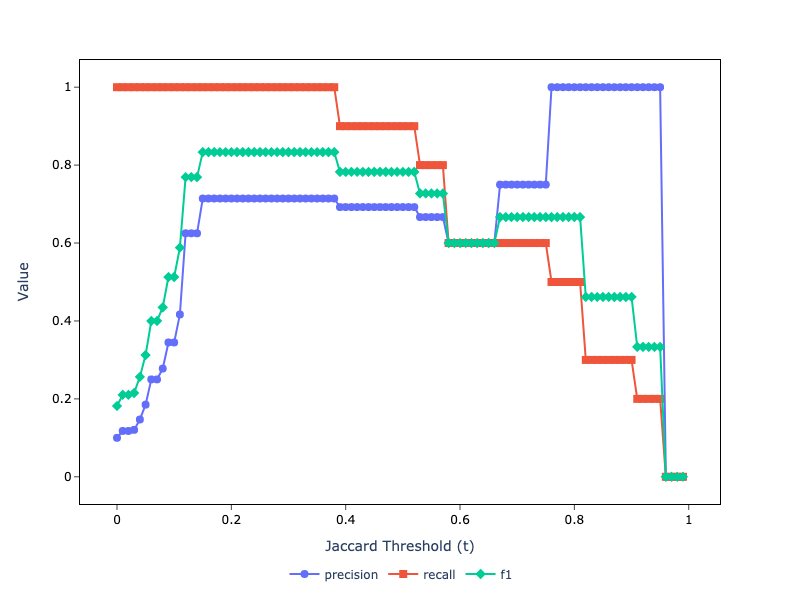
\includegraphics[width=\columnwidth]{mini-buy-fsm-main}
    \caption{Statistical metrics on `mini-buy' dataset for results of F-S model}
    \label{fig:mini-buy-fs}
\end{figure}

We can make some observations based on Figure~\ref{fig:mini-buy-fs}.
For values of $t \geq 0.78$, we end up with fewer (lower recall), but more
accurate matches (higher precision) than compared to lower values of $t$ because
the amount of false positives decreases and the amount of false negatives
increases.

For $0.6 \leq t \le 0.78$, precision decreases because the false
positive rate increases and recall increases because the false negative rate
decreases.
This is in line with expectations: the prefix becomes shorter causing a higher
percentage of attributes to be identical.
However, the prefix length is not short enough so that some of the matching
entity references in the ground truth that are more different from one another
will also be captured by \texttt{ppjoin}.

Compared to the previous interval, for values of $0.36 \leq t \le 0.6$, both
precision and recall increase compared to the previous interval.
As the prefix drops, more and more items from the ground truth are matched.
The number of false negatives decreases while the number of false positives
does not increase as fast as the number of true positives.

When $t$ is nearing zero there is an expected increase in recall due to fewer
and fewer overall negatives.
Precision, expectedly decreases due to an ever higher false positive rate.

We need to make a small note on near-identical items in the control data set,
such as \texttt{208114672} and \texttt{208114673}.
For lower values of \textit{t}, the algorithm produces two true positives and
two false positives.
By itself, the increase in false positives intuitively lowers precision.
However, lower values of \textit{t} also broaden the comparison space which
now contains entity references with short values for the name attribute,
like \texttt{205554724}.
By having new items to compare, we also increase the amount of true positives.
This dynamic ends up increasing precision as we lower values of \textit{t} so
long as we are not operating on the full input set.

Note that while we do describe the dynamic specifically for the \texttt{ppjoin}
algorithm, the dynamic of having an increased number of true positives offset
precision in an unexpected direction is not algorithm specific at all.
Regardless of the algorithm that we use, given some circumstances specific for
that algorithm, it should be possible to obtain the same effect we see here.
This observation is interesting because most entity resolution users look at the
$F_1$ score thinking that it provides a good balance between precision and recall.
These users rarely analyse the components of the $F_1$ score.
This situation can lead to unexpected outcomes.
For instance, there might be a substantial drop in $F_1$ scores, which are
indicators of accuracy, when the input data for the entity resolution process is
changed.
The reason for this is that the precision or recall may be higher than expected
for the ideal configuration determined in the controlled scenario.

On the other hand, a balanced trade-off between precision and recall might not
be a requirement.
For instance, a core legal principle applicable in many jurisdictions across the
world states that is far more favourable to let 100 guilty people escape than to
put one innocent behind bars.
By that logic, we only care about precision.
Perfect recall while still retaining some precision might be useful during
research (e.g~finding papers on the same topic) or medical diagnosis (other
cases with the same symptoms).
In these cases, sifting through false positives might be preferable to missing
out on important information because of a false negative that is due to a
suboptimal input configuration.

Our control dataset (which is purposefully flawed) instructs us that the ideal
configuration values for our algorithm are:
\begin{itemize}
    \item $0.15 \leq t \leq 0.38$ for the best balanced outcome
    \item $t \leq 0.38$ for the most sensitive system
    \item $0.76 \leq t \leq 0.95$ for the highest precision
\end{itemize}

\subsubsection{Pairwise Metrics}

The ground truth and the result of the ER process are represented as partitions
over an input set of data.
Because we include the IDs in both DG1 and DG2, the input data set will
contain 20 items.
The ground truth contains 10 pairs of items.

Measuring the similarity of two partitions can be accomplished in more ways than
measuring the statistical success of a matching process.
Among these metrics, the pairwise comparison of two partitions is the best
approximation of the statistical metrics\cite{Men10}.
Figure~\ref{fig:mini-alg-pairwise} shows the computed pairwise metrics for
various values of \textit{t}.

\begin{figure}[htbp]
    \centering
    \captionsetup{justification=centering}
    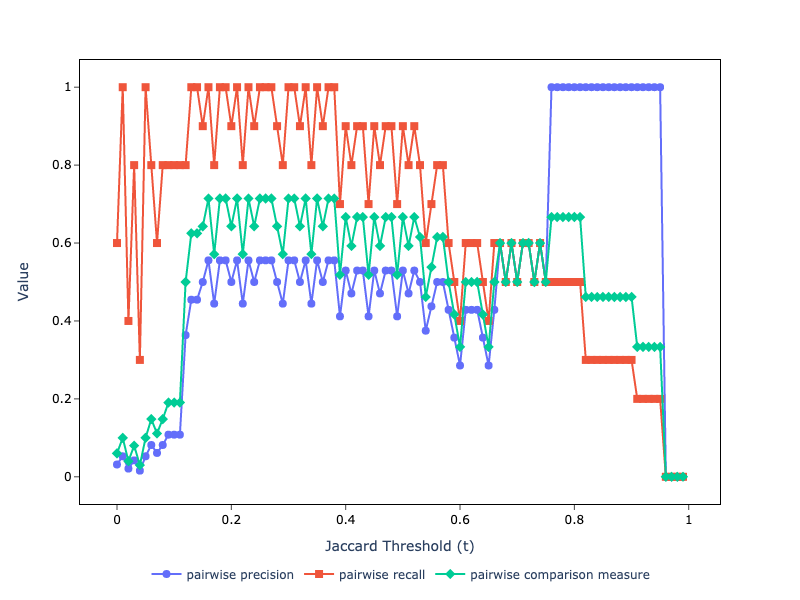
\includegraphics[width=\columnwidth]{mini-buy-algebraic-pairwise}
    \caption{Algebraic pairwise metrics on `mini-buy' dataset}\label{fig:mini-alg-pairwise}
\end{figure}

Because pairwise metrics do not support transitivity~\cite{Men10,hitesh2012},
they should be closely related to probabilistic metrics.
Indeed, we see a plot similar to the one in Figure~\ref{fig:mini-buy-fs} for statistical metrics.
The optimal configuration for a balanced entity resolution in terms of pairwise
equivalence of the result to the ground truth is very similar to the range we
observed based on probabilistic measures.
The pairwise precision plot's shape is almost identical, too.
All of these signs convince us of a successful conversion of the probabilistic
ground truth to an algebraic ground truth.

The only outlier we see is the pairwise recall plot
For $t \le 0.12$ pairwise recall drops significantly whereas statistical recall
stays at the maximum value.
The reason behind this variation lies in the difference between the two models
of entity resolution.
Whereas the standard recall formula only accounts for false negatives (of which
we can not have any using the generated data set), pairwise recall requires all
the result data to be partitioned and singleton clusters play an ever more
important part in the computed recall score as their number increases.

This situation leads to presenting our \textbf{first invariant condition
candidate}.
\textbf{Probabilistic recall seems to fail to adequately assess entity
resolution quality when the volume of data returned at the end of the entity
resolution process vastly exceeds the size of the ground truth}.
Despite encompassing all true positives, we are left with a myriad of false
positives to weed out.
This is a real problem for systems that value a result that is both accurate and
sensitive.

While in the context of our control dataset it may not seem likely that this
would raise concerns, consider that for practical applications the size of the
ideal result is often several orders of magnitude smaller than the size of the
input.
Taking into account other factors (like data cleanliness, for example), we see
that the odds of this situation occuring is not negligible at all.
Large entity resolution results are more likely to be obtained from large input
data sets than from smaller data sets, after all.

Therefore, while the input data set size certainly matters, the entity
resolution model also matters, as probabilistic recall clearly shows us.
Note that this phenomenon is dependent solely on the entity resolution model and
not on using a specific entity resolution solution to highlight it.
For other algorithms the same phenomenon may be observed depending on their
specific configuration.
Pairwise metrics seem to provide a good treatment for this phenomenon.

\subsubsection{Cluster Metrics}

Cluster metrics attempt to show how close two partitions over the same set are.
This family of metrics borrows naming from probabilistic metrics even though
the aspects being measured are quite different.
We see a plot of these cluster metrics over the `miny-buy' data set in
Figure~\ref{fig:mini-alg-cluster}.

\begin{figure}[htbp]
    \centering
    \captionsetup{justification=centering}
    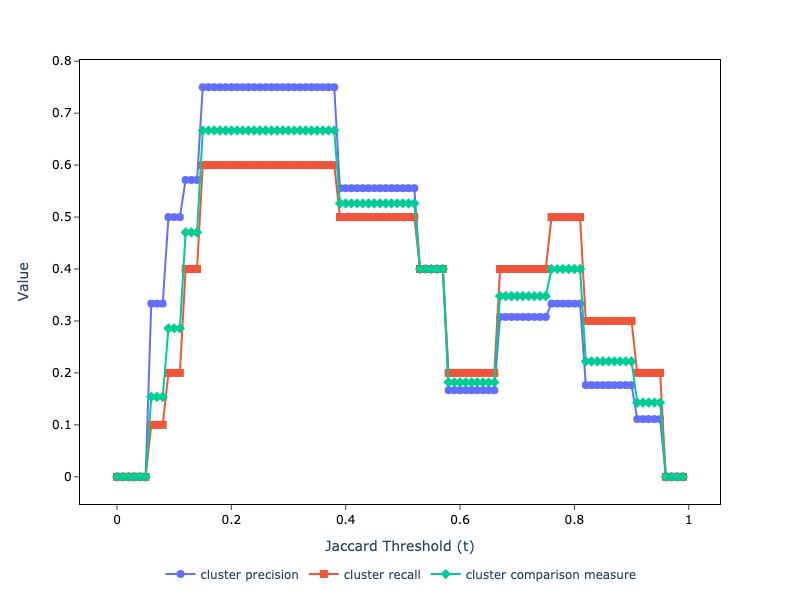
\includegraphics[width=\columnwidth]{mini-buy-algebraic-cluster}
    \caption{Algebraic cluster metrics on `mini-buy' dataset}\label{fig:mini-alg-cluster}
\end{figure}

The optimal configuration of the algorithm when balance between precision and
recall is required still consists of $0.15 \le t \le 0.38$.
We also notice that cluster metrics point out the lack of recall when \textit{t}
nears zero even more than the pairwise metrics.
This is due to singletons having a larger influence over this metric when the
sizes of the partition classes are larger (such as when duplicates abound).
Cluster recall also decreases for $0.38 \le t \le 0.58$ much more pronouncedly
than probabilistic recall or pairwise recall when partition classes are larger.

Cluster precision also has an interesting relationship with the other precision
metrics.
Take, for example, the similarity between the curves of the probabilistic and
pairwise precision and notice that the cluster precision curve is quite
different even on our control data set show in Figure~\ref{fig:mini-alg-cluster}.
As the number of singletons increases when we get fewer and fewer true positives
in the matching phase of the entity resolution process, the cluster precision
naturally drops.
In fact, we might say that \textbf{cluster precision behaves as a complement to the
other precision metrics, having higher values when the other precision metrics
have low values and lower values when the other precision metrics have high
values}.
This relationship between the three precision metrics looks like a good
candidate for our \textbf{second invariant condition}.

\subsubsection{Clustering Indexes}

Clustering indexes are, just like pairwise and cluster metrics, means to
determine the similarity of two partitions over a set.
The plots of the three indexes we want to study are in Figure~\ref{fig:mini-alg}.

\begin{figure}[htbp]
    \centering
    \captionsetup{justification=centering}
    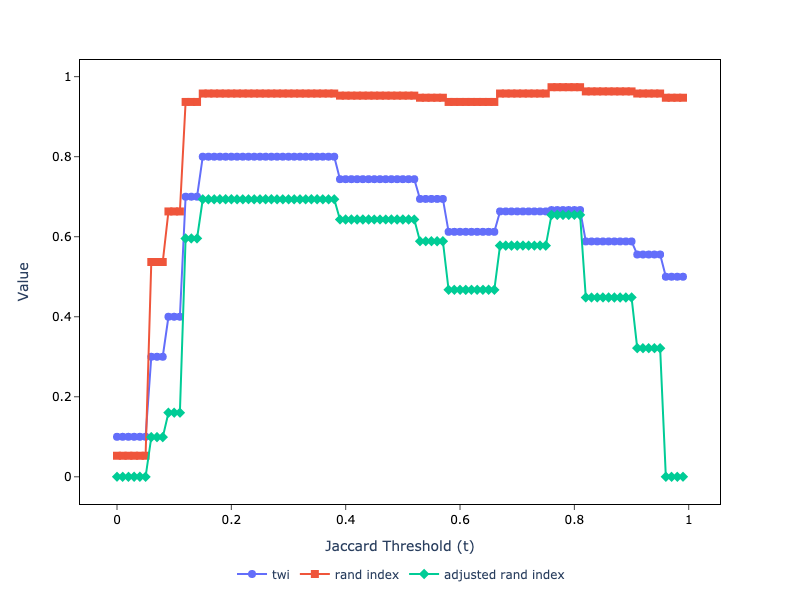
\includegraphics[width=\columnwidth]{mini-buy-algebraic-main}
    \caption{Clustering indexes on `mini-buy' dataset}
    \label{fig:mini-alg}
\end{figure}

We observe that the plot of the Adjusted Rand Index indicates both the desirable
and the undesirable values of \textit{t}.
We note that this index rates the configuration $0.76 \le t \le 0.81$ almost as
good as our running leader, $0.15 \le t \le 0.38$.
By following its plot, we should stay clear of values of \textit{t} from other
intervals.
It does a good job at identifying many of the problems spotted by precision and
cluster metrics.

By comparison with the ARI, the Rand Index is not very informative.
It signals that recall is not perfect for values of \textit{t} nearing zero and
gives its highest score for a configuration of $0.76 \le t \le 0.81$.
However, it also gives high scores for values of \textit{t} where all the other
metrics do not.

Note that even though both the Rand Index and its adjusted version are pairwise
metrics, they display plots that are more similar to the plot of the cluster
metrics.

The Talburt-Wang index's plot is a cluster-based indicator and it exhibits a
plot that has a similar shape to the ARI and the cluster metrics, albeit less
pronounced.
Compared to the ARI, it does not reveal $0.76 \le t \le 0.81$ as an interesting
configuration.

We might be able to extract a third invariant condition from the relationship
between the Talburt-Wang Index, the ARI and cluster metrics.
All of these metrics indicate the same neighbourhoods for favourable
configurations of the entity resolution algorithm.
The conjecture here is that \textbf{the best generic configuration balanced
between precision and recall of an entity resolution algorithm will be found
within the agreement area between ARI on one side and TWI or cluster metrics on
the other}.
The configuration obtained this way will be very good regardless of conditions
related to the data.
In our specific case, this means that we should expect to get the best results
using our \texttt{ppjoin} algorithm with a configuration $0.18 \le t \le 0.38$.

\subsection{Outcomes from Benchmark Datasets}\label{subsec:experiment-benchmark}

So far we have seen evidence on the controlled miniature dataset that each
theoretical model provides a lens through which we can interpret various aspects
of an entity resolution task's qualitative performance.
We have stated a few potential invariant conditions that seem to be related to
the entity resolution model more than to anything else.
By running the experiment on benchmark data we want to verify whether these
conditions are related to some attributes of the data in our control data set.

The first setup we try uses the `Abt-Buy' data set.
The plots with performance metrics for our experiment are available in Figures~\ref{fig:abt-buy-fsm-main},
~\ref{fig:abt-buy-algebraic-pairwise},~\ref{fig:abt-buy-algebraic-cluster}
and~\ref{fig:abt-buy-algebraic-main}.

\begin{figure*}[htbp]
    \begin{minipage}{0.24\textwidth}
        \centering
        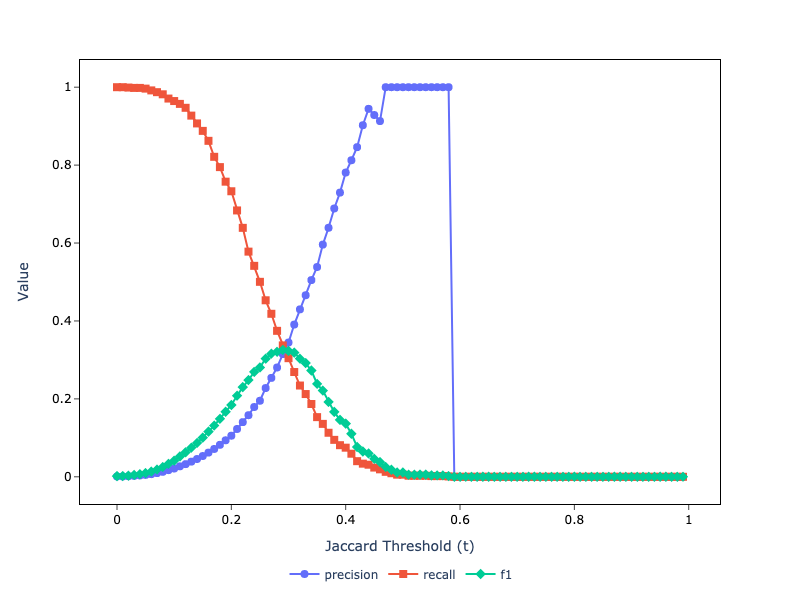
\includegraphics[width=\textwidth]{abt-buy-fsm-main}
        \caption{Abt-Buy statistical metrics.}
        \label{fig:abt-buy-fsm-main}
    \end{minipage}
    \begin{minipage}{0.24\textwidth}
        \centering
        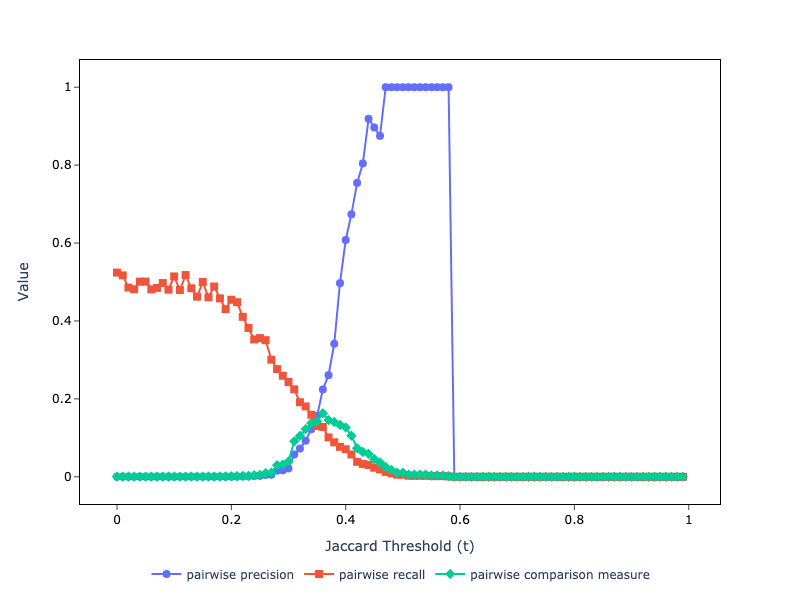
\includegraphics[width=\textwidth]{abt-buy-algebraic-pairwise}
        \caption{Abt-Buy pairwise metrics.}
        \label{fig:abt-buy-algebraic-pairwise}
    \end{minipage}
    \begin{minipage}{0.24\textwidth}
        \centering
        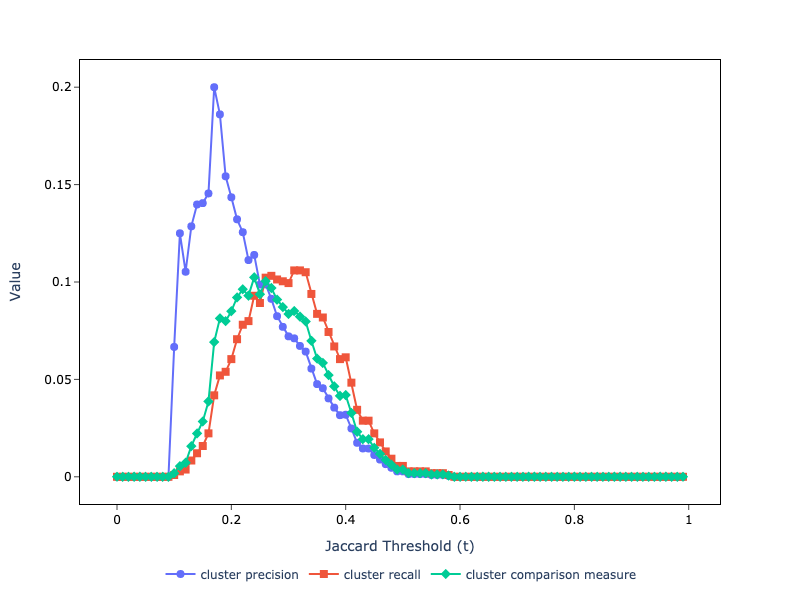
\includegraphics[width=\textwidth]{abt-buy-algebraic-cluster}
        \caption{Abt-Buy cluster metrics.}
        \label{fig:abt-buy-algebraic-cluster}
    \end{minipage}
    \begin{minipage}{0.24\textwidth}
        \centering
        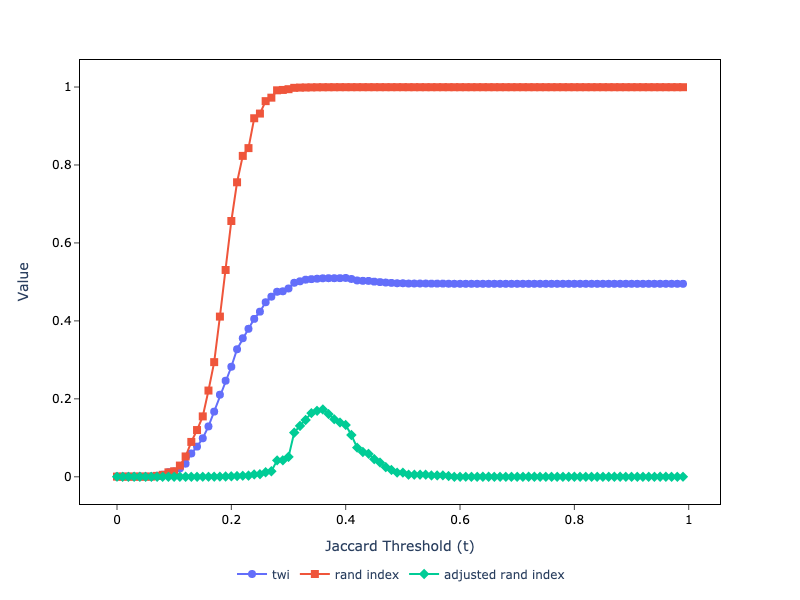
\includegraphics[width=\textwidth]{abt-buy-algebraic-main}
        \caption{Abt-Buy clustering indexes.}
        \label{fig:abt-buy-algebraic-main}
    \end{minipage}
\end{figure*}\label{abt-buy}

The invariant conditions proposed so far all hold true.
The probabilistic recall is still exceedingly high when the threshold is nearing zero and the
pairwise metrics do a good job of showing that.
Next, the cluster precision is complementary to the pairwise and probabilistic
precision.
Finally, we find the best balanced configuration between precision and recall of
$t=0.28$ is well within the target interval we envisioned at the end of the
Subsection~\ref{subsec:experiment-mini-buy} while the ARI, TWI and the cluster metrics correlate.

We move on to the `Amazon-Google Products' data set~\cite{vldb2010} and observe
the results in Figures~\ref{fig:amazon-googleproducts-fsm-main},
\ref{fig:amazon-googleproducts-algebraic-pairwise},
\ref{fig:amazon-googleproducts-algebraic-cluster} and
\ref{fig:amazon-googleproducts-algebraic-main}.

\begin{figure*}[htbp]
    \begin{minipage}{0.24\textwidth}
        \centering
        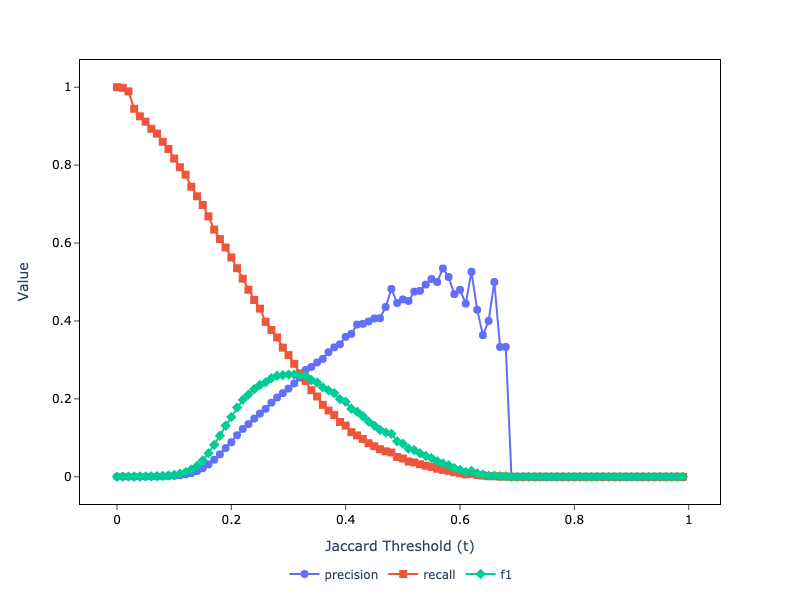
\includegraphics[width=\textwidth]{amazon-googleproducts-fsm-main}
        \caption{Amazon-Google statistical metrics.}
        \label{fig:amazon-googleproducts-fsm-main}
    \end{minipage}
    \begin{minipage}{0.24\textwidth}
        \centering
        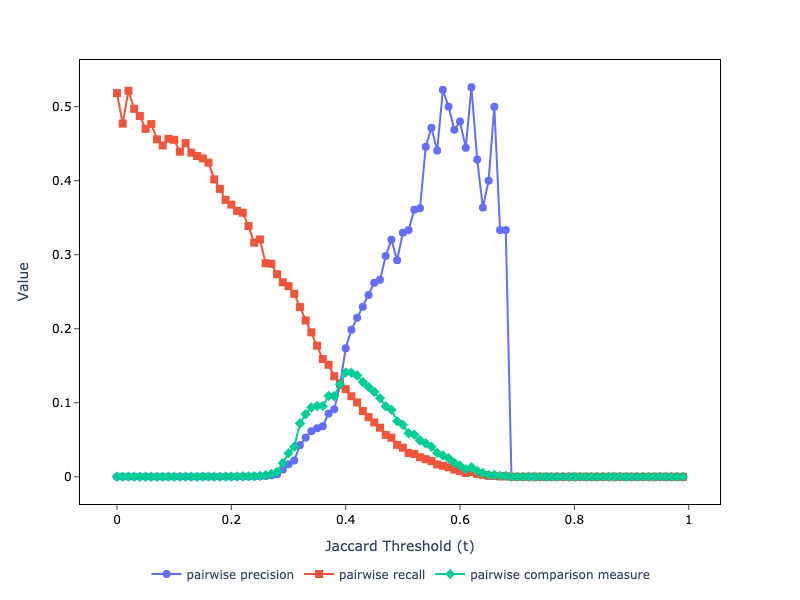
\includegraphics[width=\textwidth]{amazon-googleproducts-algebraic-pairwise}
        \caption{Amazon-Google pairwise metrics.}
        \label{fig:amazon-googleproducts-algebraic-pairwise}
    \end{minipage}
    \begin{minipage}{0.24\textwidth}
        \centering
        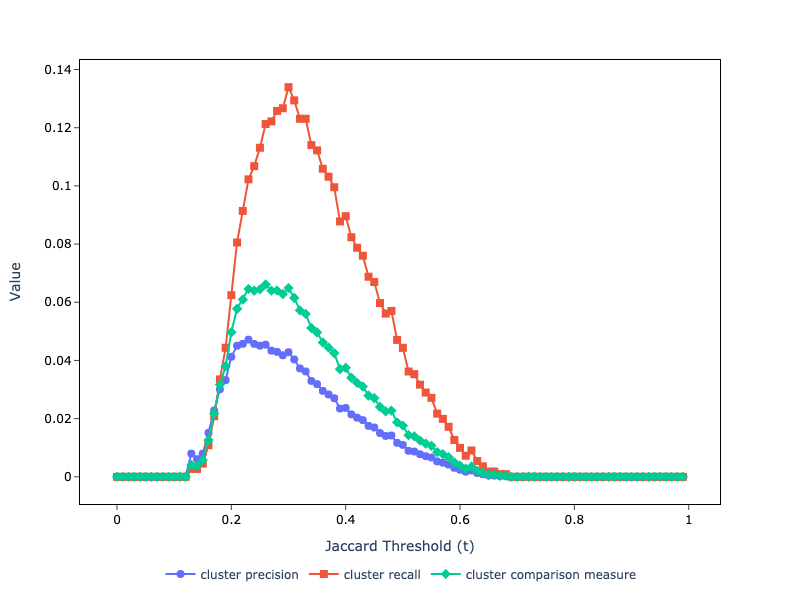
\includegraphics[width=\textwidth]{amazon-googleproducts-algebraic-cluster}
        \caption{Amazon-Google cluster metrics.}
        \label{fig:amazon-googleproducts-algebraic-cluster}
    \end{minipage}
    \begin{minipage}{0.24\textwidth}
        \centering
        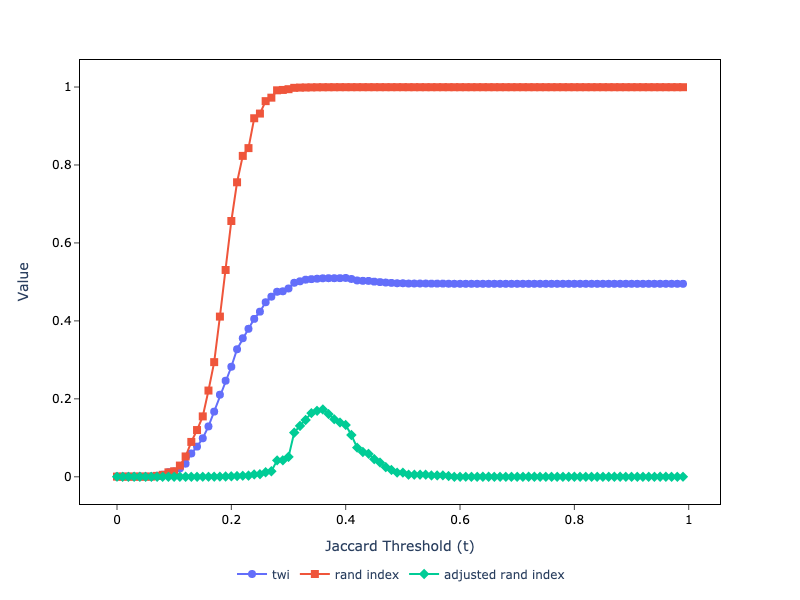
\includegraphics[width=\textwidth]{abt-buy-algebraic-main}
        \caption{Amazon-Google clustering indexes.}
        \label{fig:amazon-googleproducts-algebraic-main}
    \end{minipage}
\end{figure*}\label{amazon-google}

The picture is very similar to that painted in the experiment run on top of the
`Abt-Buy' dataset.
The probabilistic recall is very high due to an imbalance between the entity
resolution result size and the ground truth size.
The pairwise metrics are not prone to this evaluation fallacy and this is shown.
Cluster precision complements pairwise and probabilistic precision very clearly.
And, finally, the best score for entity resolution that is balanced between
probabilistic precision and recall is obtained for $t=0.3$ which is well within
the target interval.

Finally, we look at the `DBLP-ACM' benchmark dataset.
The plots we obtained after running the experiment on this dataset are available
in Figures~\ref{fig:dblp2-acm-fsm-main},
\ref{fig:dblp2-acm-algebraic-pairwise},
\ref{fig:dblp2-acm-algebraic-cluster} and
\ref{fig:dblp2-acm-algebraic-main}.

\begin{figure*}[h]
    \begin{minipage}{0.24\textwidth}
        \centering
        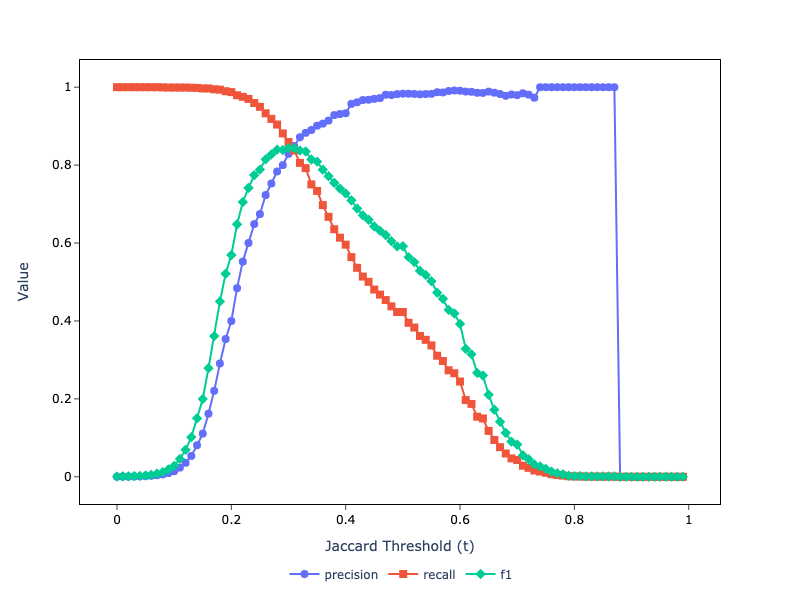
\includegraphics[width=\textwidth]{dblp2-acm-fsm-main}
        \caption{DBLP-ACM statistical metrics.}
        \label{fig:dblp2-acm-fsm-main}
    \end{minipage}
    \begin{minipage}{0.24\textwidth}
        \centering
        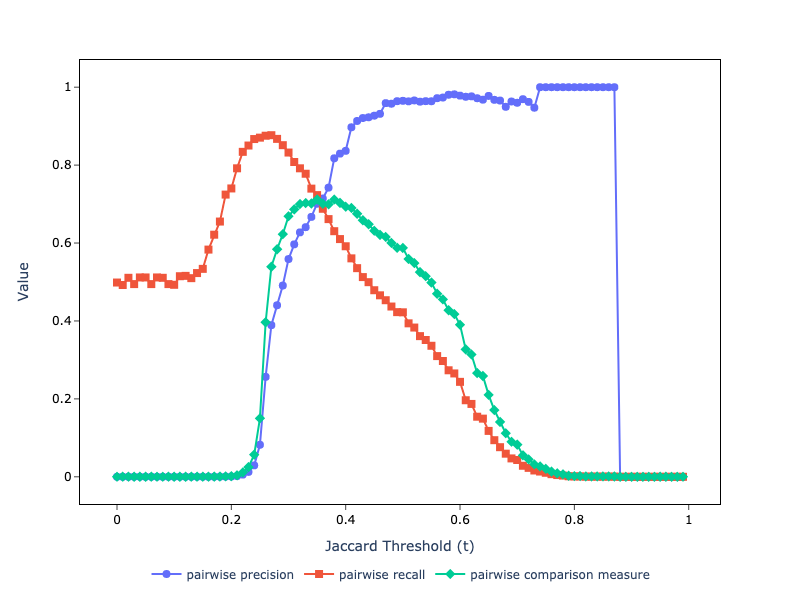
\includegraphics[width=\textwidth]{dblp2-acm-algebraic-pairwise}
        \caption{DBLP-ACM pairwise metrics.}
        \label{fig:dblp2-acm-algebraic-pairwise}
    \end{minipage}
    \begin{minipage}{0.24\textwidth}
        \centering
        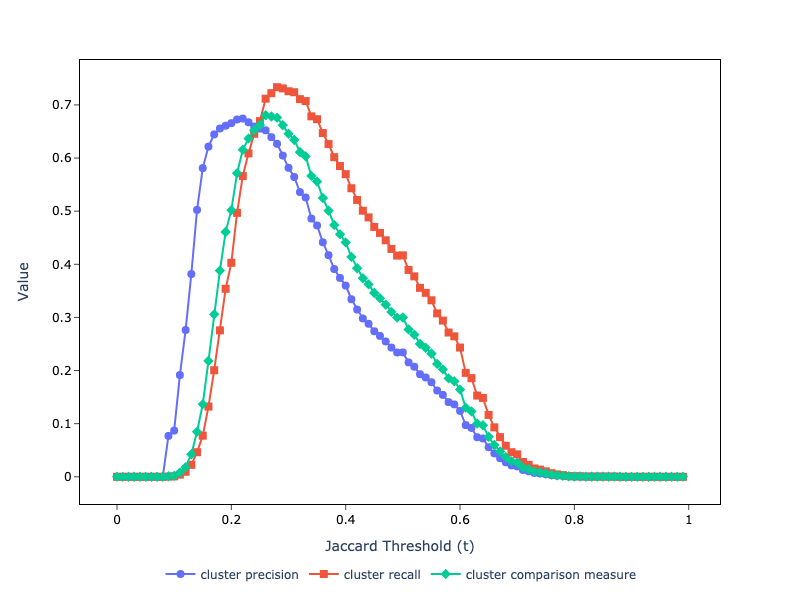
\includegraphics[width=\textwidth]{dblp2-acm-algebraic-cluster}
        \caption{DBLP-ACM cluster metrics.}
        \label{fig:dblp2-acm-algebraic-cluster}
    \end{minipage}
    \begin{minipage}{0.24\textwidth}
        \centering
        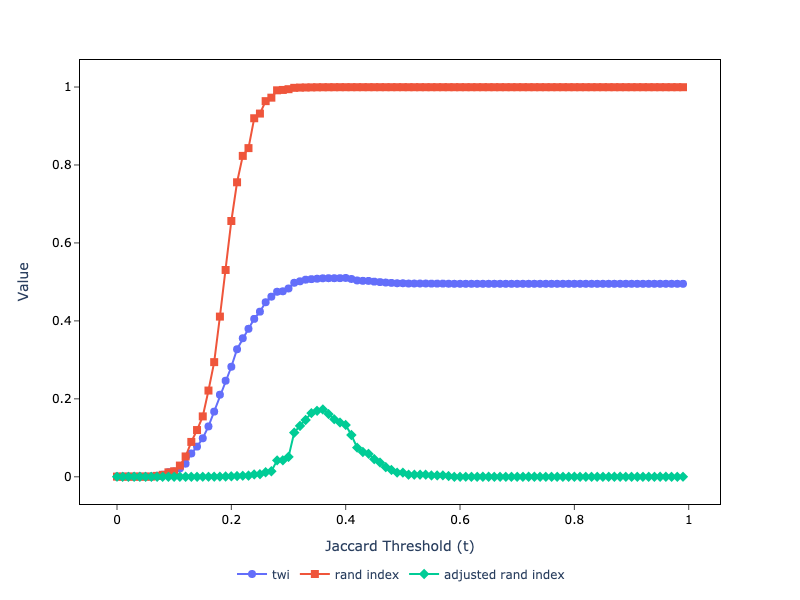
\includegraphics[width=\textwidth]{abt-buy-algebraic-main}
        \caption{DBLP-ACM clustering indexes.}
        \label{fig:dblp2-acm-algebraic-main}
    \end{minipage}
\end{figure*}\label{dblp2-acm}

Probabilistic recall is almost twice as high as pairwise recall, even though
they have the same plot.
Cluster precision is again very high where probabilistic precision and
pairwise precision are very low.
The configuration $t=0.32$ which has the highest $F_1$ score is still within the
interval predicted on our control data set.

Running the experiments has also proven to be a source of insight into the
computational expenditure surrounding entity resolution itself as well as the
calculation of entity resolution metrics.
This prompts a closer look into finding a balance between high quality outcomes
and the quantitative performance of the entity resolution solution.